\section*{Informations générales}
 
\begin{table}[h]
\centering
	\begin{tabularx}{16.8cm}{|X|X|}
	\hline
	Numéro de l'opportunité & Type d'opportunité \\
	\hline
	004 & Bonne communication client \\
	\hline
	\end{tabularx}
\end{table}

\begin{table}[h]
\centering
	\begin{tabularx}{16.8cm}{|X|X|X|}
	\hline
	Date & Visa du \RQ & Visa du \CP \\
	\hline
	 27/01/16 & pgpic & pgpic \\
	\hline
	\end{tabularx}
\end{table}

\begin{table}[h]
\centering
	\begin{tabularx}{16.8cm}{|X|X|X|X|}
	\hline
	Pilote & Activité WBS & Compte WBS & Phase d'apparition \\
	\hline
	 \Florian & Suivre les Risques et Opportunités & 1.2.3.2 & Tout au long du projet.\\
	\hline
	\end{tabularx}
\end{table}

\section*{Description du risque}

\subsection*{Résumé}
	Une bonne communication avec le client peut entrainer une meilleure compréhension de ses besoins. Cela peut permettre à l'équipe \PICCourt de mieux répondre aux exigences du client et d'éviter d'éventuels retards dans les livraisons. \\
        La bonne communication avec le client peut être due à une bonne gestion des différents outils de communication ou une bonne réactivité de sa part.
	
\subsection*{Analyse des causes}
	voir figure.

\subsection*{Criticité}

\begin{table}[h]
\centering
	\begin{tabularx}{12.8cm}{|>{
	%\columncolor{gray!40}
	}X|X|}
	\hline
	Bénéfice & 3\\
	\hline
	Probabilité & 3\\
	\hline
	Criticité & Important\\
	\hline
	\end{tabularx}
\end{table}
\newpage

\section*{Actions}
\subsection*{Actions proactives}

%\begin{table}[H]
\centering
	\begin{longtable}{|p{7cm}|p{7cm}|}
	\hline
	Cause & Actions proactives \\
	\hline
	 Se faire comprendre par le client & \begin{itemize}
	 	\item S'adapter aux connaissances du client.
	 	\item Ne pas employer de vocabulaire trop spécifique.
	 \end{itemize} \\
	\hline
	Respecter ses engagements et promesses & \begin{itemize}
		\item Ne pas se surestimer.
		\item Etre franc avec le client.
	\end{itemize} \\
	\hline
	Bonne gestion des outils de communication & \begin{itemize}
		\item Désigner un responsable de ces différents outils.
	\end{itemize} \\
	\hline
	Gérer sa communication & \begin{itemize}
		\item Ne pas se précipiter.
		\item Se maîtriser et se préparer.
	\end{itemize} \\
	\hline
	Choix pertinents des outils de communication & \begin{itemize}
		\item Rechercher les outils les plus adaptés.
		\item Tester différents outils.
	\end{itemize} \\
	\hline
	Bonne maîtrise des outils de communication & \begin{itemize}
		\item Former les membres de l'équipe à l'utilisation des ces outils
	\end{itemize} \\
	\hline
	Etre proche du client & \begin{itemize}
		\item Prendre contact régulièrement avec le client.
		\item Prendre en compte les remarques du client.
	\end{itemize} \\
	\hline
	Mise en place d'outils de communication performants & \begin{itemize}
		\item Rechercher les outils les plus adaptés
		\item Tester différents outils
	\end{itemize} \\
	\hline
	\end{longtable}
%\end{table}

\section*{Décision de clôture}
Par le \CP{} et le pilote du risque.
\begin{table}[h]
\centering
	\begin{tabularx}{16.8cm}{|X|X|}
	\hline
	Date de clôture & Raison de la clôture \\
	\hline
	  & \\
	\hline
	\end{tabularx}
\end{table}

\section*{Historique des modifications}
\begin{table}[h]
\centering
	\begin{tabularx}{16.8cm}{|X|X|}
	\hline
	Date & Modification \\%\rowcolor{gray!40} 
	\hline
	  & \\
	\hline
	\end{tabularx}
\end{table}
\newpage


\begin{figure}
	\centering
	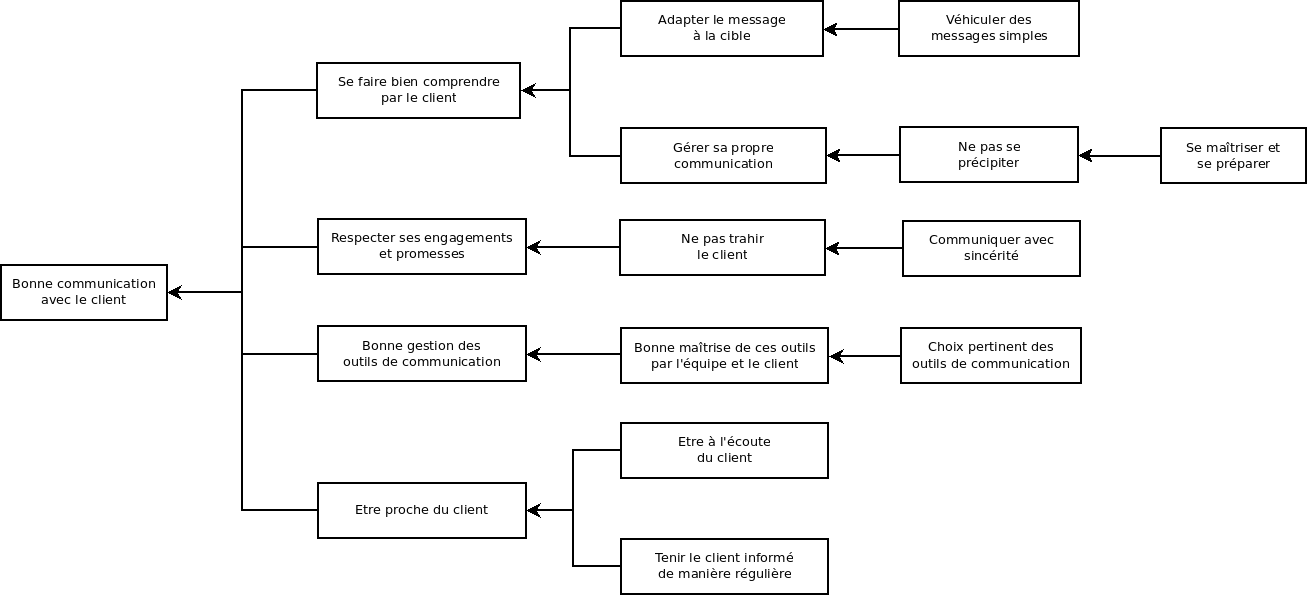
\includegraphics[scale=0.5, angle=90]{../images/AnalyseOpportunite_nPourquoi_FDO004.png}
\end{figure}